\chapter{Experimental results}

To compare the four presented approaches, we generated benchmark datasets and ran all the algorithms on them. In this chapter, we present the results.

\section{Commute dataset}

The used dataset contains 100 passenger requests. Each customer group departs from a random location in Pilsen and travels to a random location in Prague. The distance between the two cities is approximately 90 kilometers. The departure times are randomly distributed in a four-hour time window. Each group is between 1 and 10 people. The depot is set in Prague. It is important to note that the first group in each route gets always picked up on time. This means that the location of the depot has no effect on the group's delays; setting it far from the departure area does, however, make using more buses more costly. The available bus type can take up to 80 persons, its operating cost per kilometer is $80$, and its fixed cost for rental is $50000$.

All the algorithms use the same fitness function, with the delay penalty constant equaling $0.01$.

All the genetic algorithms have a population size set to $30$ individuals, with $3$ best individuals (\textit{elites}) passed from the old to the new population. All the encodings also require an upper limit to the number of buses used, which we set to $30$ buses. The \textit{ACO} uses \textit{20} ants, meaning that 20 new solutions are generated in each iteration. Other parameters are set as described in sections \ref{sec:genetic_hyperparams} and \ref{sec:aco_hyperparams}.

The algorithms ran for exactly 80 minutes, after which they were terminated. Figure \ref{fig:exp_commute} shows the progression of the best fitness value found by each approach. The experiments were repeated 10 times. The value shown is the mean fitness of the 10 runs, with the first and third quartiles depicted by the translucent region. The figure shows progression in time and has both the x and y axis on a logarithmic scale.

\begin{figure}[b]
    \centering
    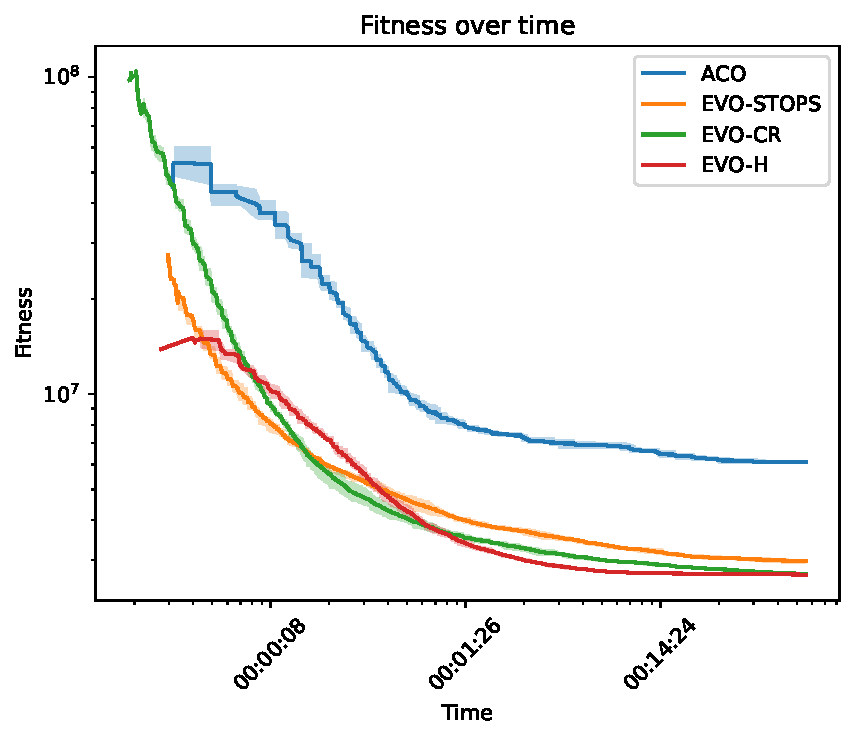
\includegraphics
    {img/exp_commute_100_time.pdf}
    \caption{Commute dataset - fitness values in time}
    \label{fig:exp_commute}
\end{figure}

Table \ref{tab:exp_commute_route_stats} shows the basic information about the best solution returned by each algorithm - how much all the routes cost, how many kilometers were traveled in total, and how many buses were used. 

\begin{table}
    \centering
    \begin{tabular}{lcccccc}
         & Total costs & Km traveled & Buses used \\
         \hline
         EVO-STOPS & 2231202.82 & 9140.035 & 30 \\
         EVO-CR & \textbf{2153207.33} & 8790.092 & \textbf{29} \\
         EVO-H & 2160139.18 & 8876.740 & \textbf{29} \\
         ACO & 2164447.95 & \textbf{7680.599} & 31 \\
    \end{tabular}
    \caption{Commute dataset - Route statistics}
    \label{tab:exp_commute_route_stats}
\end{table}

Table \ref{tab:exp_commute_delay_stats} shows the statistics about the group's delays - the delay of the most delayed group and the average and median delay of all the groups.

\begin{table}
    \centering
    \begin{tabular}{lcccccc}
         &  Maximum delay & Average delay & Median delay \\
         \hline
         EVO-STOPS & 1963.7 & 658.1 & 672.2 \\
         EVO-CR & 1682.4 & 601.4 & \textbf{590.6} \\
         EVO-H & \textbf{1553.4} & \textbf{595.1} & 596.5 \\
         ACO & 5207.0 & 1537.0 & 1380.9 \\
    \end{tabular}
    \caption{Commute dataset - Delay statistics}
    \label{tab:exp_commute_delay_stats}
\end{table}

When examining the results, we see that no approach is strictly better than all the others. While the Ant Colony Optimization managed to find the shortest set of routes, it failed to deliver the groups in time, with four groups arriving at their destination more than an hour later than if they took a car or a taxi. The \textit{EVO-STOPS} approach returned the solution with the highest total costs and otherwise mediocre results. The \textit{EVO-CR} and \textit{EVO-H} approaches returned very similar results on all fronts.